
% specify the document type
\documentclass{beamer}
\usepackage[utf8]{inputenc}
\setbeamertemplate{bibliography item}{\insertbiblabel}

% specify beamer theme stuff
\usetheme{Copenhagen}
\usecolortheme{beaver}
\usefonttheme{professionalfonts}

% include a set of useful packages
\usepackage{graphicx}
\usepackage{amsmath}
\usepackage{amssymb}
\usepackage{cancel}
\usepackage{algorithm2e}
\usepackage{float}
\usepackage{caption}
\usepackage{fancyvrb}
\usepackage[toc,page]{appendix}
\usepackage{hyperref}
\usepackage{subfig}
\usepackage{color}
\usepackage[export]{adjustbox}
\usepackage{multicol}

% define some useful commands
\newcommand{\bvec}[1]{\boldsymbol{#1}}

% setup paths for images
\graphicspath{ {../images/} }

%
% start the presentation
%

% define the title stuff
\title{QBX and the DPIE for the Maxwell Equations}
\author{Christian Howard}
\institute{University of Illinois @ Urbana-Champaign}
\date{Fall 2017 - CS 598 APK}

% begin the actual document
\begin{document}
	
	% throw in the title page
	\frame{\titlepage}
	
	% project goal
	\begin{frame}
	\frametitle{The Goal}
	For this project, the goals were to implement a model for the Python package \textbf{pytential} for tackling the Maxwell Equations for perfect conductors using QBX and the Decoupled Potential Integral Equation (DPIE) formulation. The main expectation with using this model, versus the Magnetic Field Integral Equation (MFIE), is better resolution and convergence across different frequencies.
	
	
\end{frame}
	
	% slides talking about motivation
	\begin{frame}
	\frametitle{A Little Context}
	Building cool stuff like radars, missiles antennas, medical imaging tech, and more benefit a lot from solving the Maxwell Equations to solve some tough Computational Electromagnetics problems
	
	\vspace{0.5in}
	\hfil\hfil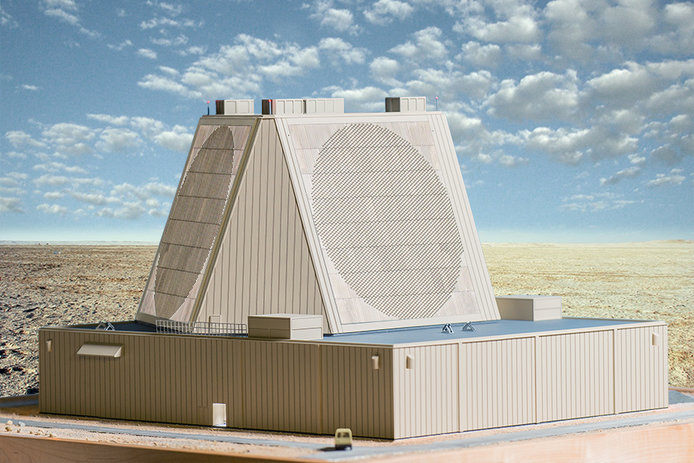
\includegraphics[width=5cm,frame]{raytheonRadar}\hfil\hfil
	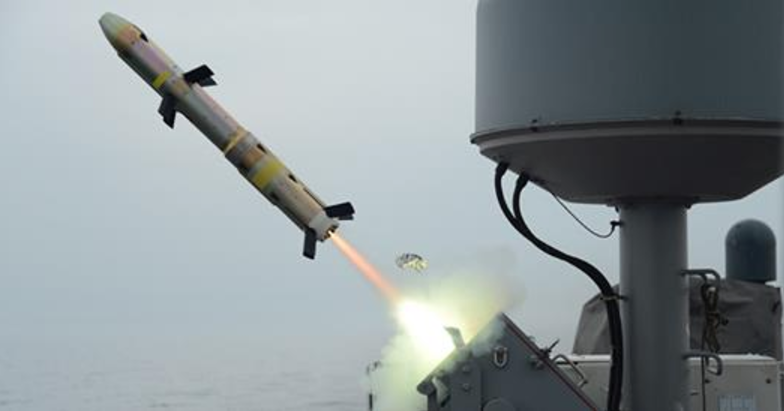
\includegraphics[width=5cm,frame]{griffinMissile}\newline
	\null\hfil\hfil\makebox[5cm]{Early Warning Radar}
	\hfil\hfil\makebox[5cm]{Raytheon AGM-176 Griffin}
	
	\end{frame}

	\begin{frame}
	\frametitle{Industry needs Robustness and Efficiency}
	For people in industry working on systems that can be modeled with Partial Differential Equations, there are a few key features for a solver that will make it more likely to be adopted:
	
	\begin{itemize}
		\item Solver must be fast
		\item Solver must be accurate
		\item Solver must be robust 
	\end{itemize}

	\vspace{0.1in}
	\begin{center}
		
\includegraphics[width=5cm,frame]{likeDuh}
	\end{center}
	\end{frame}

	\begin{frame}
	\frametitle{Industry needs Robustness and Efficiency}
	Those demands are lofty. Fortunately, Integral Equation based solvers make hitting all those targets feasible. Using Integral Equation based solvers, we can get the following:
	
	\begin{itemize}
		\item Excellent convergence rates
		\item Excellent conditioning properties
		\item Ability to accelerate computations using the Fast Multipole Method (FMM) and other hierarchical algorithms
	\end{itemize}
	\end{frame}

	% Dive into Maxwell Equation Formulation - MFIE
	\begin{frame}
	\frametitle{Electromagnetic Scattering on Perfect Conductors}
	Many problems can be approximated as electromagnetic scattering with perfect conductors, so modeling these problems is our goal. Discussion on the modeling in the slides to come is based on \cite{dpie}.
	
	\vspace{0.1in}
	\begin{center}
		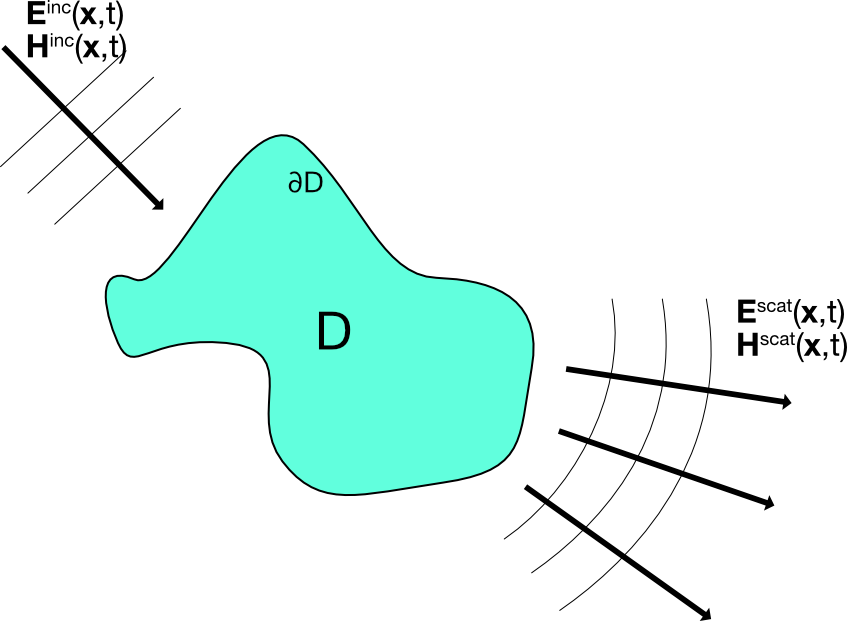
\includegraphics[width=7cm]{scatter_problem_pic}
	\end{center}
	\end{frame}
	
	\begin{frame}
	\frametitle{Electromagnetic Scattering on Perfect Conductors}
	For a fixed frequency $\omega$, the electric and magnetic fields, $\mathcal{E}$ and $\mathcal{H}$, take the form:
	
	\begin{align*}
	\mathcal{E}(\bvec{x},t) &= \mathcal{R}\lbrace \bvec{E}(\bvec{x}) e^{- i \omega t}\rbrace \\
	\mathcal{H}(\bvec{x},t) &= \mathcal{R}\lbrace \bvec{H}(\bvec{x}) e^{- i \omega t}\rbrace
	\end{align*}
	
	where $\mathcal{R}\lbrace z \rbrace$ returns the real part of $z$. We can then represent $\bvec{E}(\bvec{x})$ and $\bvec{H}(\bvec{x})$ as a sum of incident (known) and scattered (unknown) fields:
	
	\begin{align*}
	\bvec{E} &= \bvec{E}^{inc} + \bvec{E}^{scat} \\
	\bvec{H} &= \bvec{H}^{inc} + \bvec{H}^{scat}
	\end{align*}
	
	\end{frame}

	
	\begin{frame}
	\frametitle{Electromagnetic Scattering on Perfect Conductors}
	The equations to be solved take the form:
	
	\begin{itemize}
		\item Maxwell Equations
		\begin{align*}
		\nabla \times \bvec{E} = i \omega \mu \bvec{H}, \;\nabla \times \bvec{H} = - i \omega \epsilon \bvec{E}
		\end{align*}
		%
		\item Sommerfield-Silver-Müller Radiation Condition
		\begin{align*}
		\bvec{H}^{scat}(\bvec{x}) \times \frac{\bvec{x}}{|\bvec{x}|} - \sqrt{\frac{\mu}{\epsilon}} \bvec{E}^{scat}(\bvec{x}) = o(|\bvec{x}|^{-1}), \;\; |\bvec{x}| \rightarrow \infty
		\end{align*}
		%
		\item Perfect Conductor Boundary Conditions
		\begin{align*}
		\left(\bvec{n} \times \bvec{E}^{scat} \right)|_{\partial D} &= -\left( \bvec{n} \times \bvec{E}^{inc} \right)|_{\partial D} \\
		\left(\bvec{n} \cdot \bvec{H}^{scat} \right)|_{\partial D} &= -\left( \bvec{n} \cdot \bvec{H}^{inc} \right)|_{\partial D} 
		\end{align*}
	\end{itemize}
	
	\end{frame}

	\begin{frame}
	\frametitle{Electromagnetic Scattering on Perfect Conductors}
	Some other useful relationships for modeling the problem are
	
		\begin{align*}
		\left(\bvec{n} \cdot \bvec{E} \right)|_{\partial D} &= \frac{\rho}{\epsilon}|_{\partial D} \\
		\left(\bvec{n} \times \bvec{H} \right)|_{\partial D} &= \bvec{J}|_{\partial D} \\
		\nabla_s \cdot \bvec{J} &= i \omega \rho
		\end{align*}

	where $\bvec{J}$ and $\rho$ are the induced current density and charge on $\partial D$ and $\nabla_s \cdot \bvec{J}$ represents the surface divergence of the tangential current density.

	\end{frame}


	\begin{frame}
	\frametitle{Magnetic Field Integral Equation}
	The Magnetic Field Integral Equation (MFIE) can be used to model electromagnetic scattering for perfect conductors. The formulation begins by defining $\bvec{E}^{scat}$ and $\bvec{H}^{scat}$ using the Lorenz gauge vector and scalar potentials, $\bvec{A}^{scat}$ and $\phi^{scat}$
	
	\begin{align*}
	\bvec{E}^{scat} &= i \omega \bvec{A}^{scat} - \nabla \phi^{scat} \\
	\bvec{H}^{scat} &= \frac{1}{\mu} \nabla \times \bvec{A}^{scat}
	\end{align*}
	
	with the Lorenz gauge relationship defined as
	
	\begin{align*}
	\nabla \cdot \bvec{A}^{scat} &= i \omega \mu \epsilon \phi^{scat}
	\end{align*}
	
	\end{frame}

	\begin{frame}
	\frametitle{Magnetic Field Integral Equation}
	We then define the $\bvec{A}^{scat}$ and $\phi^{scat}$ based on the induced surface current $\bvec{J}$ and charge $\rho$ using Single Layer Potentials in the following manner:
	
	\begin{align*}
	\bvec{A}^{scat}[\bvec{J}](\bvec{x}) &= \mu S_k [\bvec{J}](\bvec{x}) & \equiv \mu \int_{\partial D} g_k(\bvec{x} - \bvec{y}) \bvec{J}(\bvec{y})dA_y \\
	\bvec{\phi}^{scat}[\rho](\bvec{x}) &=\frac{1}{\epsilon} S_k [\rho](\bvec{x}) & \equiv \frac{1}{\epsilon} \int_{\partial D} g_k(\bvec{x} - \bvec{y}) \rho(\bvec{y})dA_y
	\end{align*}
	
	with $k = \omega \sqrt{\epsilon \mu}$ and the kernel being defined as:
	
	\begin{align*}
	g_k(\bvec{x}) &= \frac{e^{i k |\bvec{x}|}}{4 \pi |\bvec{x}|}
	\end{align*}
	
	\end{frame}


	\begin{frame}
	\frametitle{Magnetic Field Integral Equation}
	Using $\bvec{H}^{scat} = \frac{1}{\mu} \nabla \times \bvec{A}^{scat}$ and the boundary condition
	
	\begin{align*}
	\left.\left(\bvec{n} \times \bvec{H} \right)\right|_{\partial D} &= \left.\bvec{J}\right|_{\partial D}
	\end{align*}
	
	the Magnetic Field Integral Equation can be found to be the following:
	
	\begin{align*}
	\frac{1}{2} \bvec{J}(\bvec{x}) - K[\bvec{J}](\bvec{x}) &= \bvec{n}(\bvec{x}) \times H^{inc}(x), \;\; \bvec{x} \in \partial D \\
	K[\bvec{J}](\bvec{x}) &= \int_{\partial D} \bvec{n}(\bvec{x}) \times \nabla \times g_k(\bvec{x} - \bvec{y}) \bvec{J}(\bvec{y}) dA_y \\
	\end{align*}
	
	\end{frame}

	\begin{frame}
	\frametitle{Magnetic Field Integral Equation}
	After obtaining $\bvec{J}$, one can obtain $\rho$ via the continuity equation
	
	\begin{align*}
	\nabla_s \cdot \bvec{J} &= i \omega \rho
	\end{align*}
	
	where $\nabla_s \cdot \bvec{J}$ represents the surface divergence of the tangential current density. Alternatively, you can back out $\phi^{scat}$ using the Lorenz gauge relationship:
	
	\begin{align*}
	\phi^{scat} &= -\frac{i}{\omega \epsilon} \nabla \cdot S_k[\bvec{J}]
	\end{align*} 
	
	From here, obtaining $\bvec{E}^{scat}$ and $\bvec{H}^{scat}$ is straight forward.
	
	\end{frame}


	\begin{frame}
	\frametitle{Problems with MFIE}
	The MFIE is ill conditioned as $\omega \rightarrow 0$. To back out $\bvec{E}^{scat}$ and $\bvec{H}^{scat}$, need to perform computations with $\omega^{-1}$ which leads to catastrophic cancellation. For example, $\rho$ is computed by
	
	\begin{align*}
	\rho &= \frac{\nabla_s \cdot \bvec{J}}{i \omega \epsilon}
	\end{align*}
	
	Additionally, for $\omega = 0$ in multiply-connected domains, MFIE has a nonzero nullspace dimensionality equivalent to the genus of $\partial D$
	
	\end{frame}
	
	% looking at the DPIE
	\begin{frame}
	\frametitle{The Decoupled Potential Integral Equation}
	The premise for this formulation is to impose boundary conditions on the potentials $\phi$ and $\bvec{A}$ instead of the fields $\bvec{E}$ and $\bvec{H}$, in hopes the resulting integral equation can be better conditioned, insensitive to the topology of the domain, and remain straight forward to solve.
	
	\vspace{0.1in}
	\begin{center}
		
\includegraphics[width=4cm,frame]{gotInteresting}
	\end{center}
	\end{frame}

	\begin{frame}
	\frametitle{The Decoupled Potential Integral Equation}
	First, the boundary conditions that will be imposed on the vector and scalar potentials are the following:
	
	\begin{align*}
	\left. \left(\bvec{n} \times \bvec{A}^{scat}\right)\right|_{\partial D} &= - \left. \left(\bvec{n} \times \bvec{A}^{inc}\right)\right|_{\partial D} \\
	\left. \left(\bvec{n} \times \nabla \phi^{scat}\right)\right|_{\partial D} &= - \left. \left(\bvec{n} \times  \nabla \phi^{inc}\right)\right|_{\partial D} \\
	\end{align*}
	
	These boundary conditions for the potentials can be shown to satisfy the Maxwell equations, radiation condition, and perfect conductor boundary conditions.
	\end{frame}

	\begin{frame}
	\frametitle{The Decoupled Potential Integral Equation}
	Next is important to note that the Lorenz gauge condition does not uniquely determine what form the potentials $\bvec{A}$ and $\bvec{\phi}$ take. Due to this, $\bvec{A}$ and $\bvec{\phi}$ can be chosen to cast the problem into a more ideal form. For an incoming plane wave with a polarization vector $\bvec{E}_p$ and propagation direction $\bvec{u}$, the incident fields can be written as
	
	\begin{align*}
	\bvec{E}^{inc} &= \bvec{E}_p e^{i k \bvec{u} \cdot \bvec{x}} \\
	\bvec{H}^{inc} &= \sqrt{\frac{\epsilon}{\mu}} \bvec{u} \times \bvec{E}_p e^{i k \bvec{u} \cdot \bvec{x}}
	\end{align*}
	
	The standard potentials are $\bvec{A}^{inc} = \frac{\bvec{E}^{inc}}{i \omega}$, $\phi^{inc} = 0$, but these can be modified to the stable form
	
	\begin{align*}
	\bvec{A}^{inc} &= - \bvec{u} \left( \bvec{x} \cdot \bvec{E}_p\right) \sqrt{\mu \epsilon} e^{i k \bvec{u} \cdot \bvec{x}} \\
	\phi^{inc} &= - \bvec{x} \cdot \bvec{E}_p e^{i k \bvec{u} \cdot \bvec{x} }
	\end{align*}
	
	\end{frame}

	\begin{frame}
	\frametitle{The Decoupled Potential Integral Equation}
	To  handle uniqueness of the vector potential solution $\bvec{A}^{scat}$ for all $k \geq 0$, the scalar Helmholtz is modified to
	
	\begin{align*}
	\Delta \phi^{scat} + k^2 \phi^{scat} &= 0 \\
	\phi^{scat}|_{\partial D_j} &= f + V_j \\
	\int_{\partial D_j} \left( \nabla \phi^{scat} \cdot \bvec{n}\right) ds &= Q_j
	\end{align*}
	
	where $f|_{\partial D_j} = - \phi^{inc}|_{\partial D_j}$ and $Q_j = - \int_{\partial D_j} \left( \nabla \phi^{inc} \cdot \bvec{n}\right) ds$
	
	\end{frame}

	\begin{frame}
	\frametitle{The Decoupled Potential Integral Equation}
	To handle uniqueness of the vector potential solution $\bvec{A}^{scat}$ for all $k \geq 0$, the vector Helmholtz is modified to
	
	\begin{align*}
	\Delta \bvec{A}^{scat} + k^2 \bvec{A}^{scat} &= 0 \\
	\left(\bvec{n} \times \bvec{A}^{scat}\right)|_{\partial D} &= \bvec{f} \\
	\bvec{n} \cdot \bvec{A}^{scat}|_{\partial D_j} &= h + v_j \\
	\int_{\partial D_j} \left( \bvec{n} \cdot \bvec{A}^{scat} \right) ds &= q_j
	\end{align*}
	
	where $\bvec{f}|_{\partial D_j} = - \bvec{n} \times \bvec{A}^{inc}|_{\partial D_j}$, $h = - \nabla \cdot \bvec{A}^{inc}|_{\partial D}$ and $q_j = - \int_{\partial D_j} \left( \bvec{n} \cdot \bvec{A}^{inc} \right) ds$
	
	\end{frame}

	\begin{frame}
	\frametitle{The Decoupled Potential Integral Equation}
	Note the following operator definitions
	
	\begin{align*}
	S_k \sigma &= \int_{\partial D} g_k (\bvec{x} - \bvec{y}) \sigma(\bvec{y}) dA_y \\
	D_k \sigma &= \int_{\partial D} \frac{\partial g_k}{\partial n_y} (\bvec{x} - \bvec{y}) \sigma(\bvec{y}) dA_y \\
	S_k^{'} \sigma &= \int_{\partial D} \frac{\partial g_k}{\partial n_x}  (\bvec{x} - \bvec{y}) \sigma(\bvec{y}) dA_y \\
	D_k^{'} \sigma &= \frac{\partial }{\partial n_x}  \int_{\partial D} \frac{\partial g_k}{\partial n_y}  (\bvec{x} - \bvec{y}) \sigma(\bvec{y}) dA_y
	\end{align*}
	
	where $g_k(\bvec{x})$ is again defined as
	
	\begin{align*}
	g_k(\bvec{x}) &= \frac{e^{i k |\bvec{x}|}}{4 \pi |\bvec{x}|}
	\end{align*}
	
\end{frame}

	\begin{frame}
	\frametitle{The Decoupled Potential Integral Equation}
	After the modification to the scalar and vector Helmholtz, the scaled DPIEs for the scalar potential is
	
	\begin{align*}
	\frac{\sigma}{2} + D_{k}\sigma - i k S_k \sigma - \sum_{j=1}^N V_j \chi_j &= f \\
	\int_{\partial D_j} \left( \frac{1}{k} D_{k}^{'} \sigma + i \frac{\sigma}{2} - i S_k^{'}\sigma \right) ds &= \frac{1}{k}Q_j
	\end{align*}
	
	with unknowns $\lbrace V_j\rbrace$, $\sigma$ for a representation of $\phi^{scat}(\bvec{x})$ as
	
	\begin{align*}
	\phi^{scat}(\bvec{x}) &= D_k [\sigma](\bvec{x}) - i k S_k [\sigma] (\bvec{x})
	\end{align*}
	
	\end{frame}

	\begin{frame}
	\frametitle{The Decoupled Potential Integral Equation}
	After the modification to the scalar and vector Helmholtz, the scaled DPIEv for the vector potential is
	
	\begin{align*}
	\frac{1}{2}\begin{pmatrix}
	\bvec{a} \\
	\rho
	\end{pmatrix}
	+ 
	\bar{L} \begin{pmatrix}
	\bvec{a} \\
	\rho
	\end{pmatrix}
	+
	i \bar{R} \begin{pmatrix}
	\bvec{a} \\
	\rho
	\end{pmatrix}
	+ \begin{pmatrix}
	\bvec{0} \\
	\sum_{j=1}^N v_j \chi_j
	\end{pmatrix}
	&= \begin{pmatrix}
	\bvec{f} \\
	\frac{h}{k}
	\end{pmatrix} \\
	\int_{\partial D_j} \left(  \bvec{n} \cdot \nabla \times S_k\bvec{a} - k \bvec{n} \cdot S_k\left(\bvec{n} \rho \right) \right) ds + \;\;\;\;\;\;\;\;\;&\\
	i \int_{\partial D_j} \left(k \bvec{n} \cdot S_k\left(\bvec{n} \times \bvec{a}\right) - \frac{\rho}{2} + S_k^{'}\rho \right) ds &= q_j
	\end{align*}
	
	with $\bar{L}$, $\bar{R}$ are defined on Slide \ref{s:dpievop} and with unknowns $\lbrace v_j\rbrace$, $\bvec{a}$, $\rho$ for a representation of $\bvec{A}^{scat}(\bvec{x})$ as
	
	\begin{align*}
	\bvec{A}^{scat}(\bvec{x}) &= \nabla \times S_k[\bvec{a}](\bvec{x}) - k S_k[\bvec{n}\rho](\bvec{x}) \\
	&\;\;\;\; + i \left(k S_k[\bvec{n} \times \bvec{a}](\bvec{x}) + \nabla S_k[\rho](\bvec{x})\right)
	\end{align*}
	
	\end{frame}


	% briefly discuss QBX
	\begin{frame}
	\frametitle{Quadrature by Expansion}
	The goal of QBX is to accurately handle evaluation of layer potential integrals on a boundary $\partial D$ where singularities can exist due to the integral operator kernel. 
	
	\hfil\hfil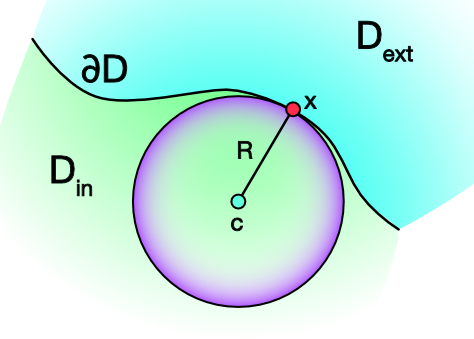
\includegraphics[width=5cm]{qbx_image}\hfil\hfil
	
	The idea is to perform an order $p$ expansion of some integral operator $K \sigma (\bvec{x})$ from some location $\bvec{c}$ and used that to evaluate $K \sigma(\bvec{x})$ at some boundary location $\bvec{x}$ where a singularity might exist. Given the field is smooth when restricted to the interior or exterior of the domain, this method is robust and accurate \cite{qbx}.
	
	\end{frame}

	\begin{frame}
	\frametitle{Quadrature by Expansion}
	Using QBX, one can create robust and accurate discretizations of integral equations to solve for unknown densities and evaluating layer potentials for any representations one cares about. 
	
	\vspace{0.1in}
	\begin{center}
		
\includegraphics[width=6cm]{qbxAwesome}
	\end{center}
	\vspace{0.1in}
	
	In the context of solving the DPIE system of integral equations, this method is worthwhile to use for both its robustness and accuracy properties.
	\end{frame}


	% briefly discuss QBX
	\begin{frame}
	\frametitle{Numerical Results}
	\hfil\hfil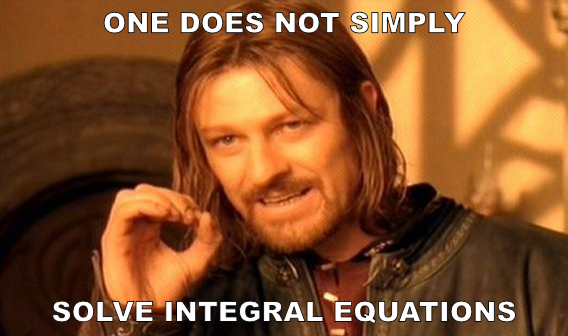
\includegraphics[width=8cm,frame]{notSimplySolveIE}\hfil\hfil
	\end{frame}


	\begin{frame}
	\frametitle{Questions}
	\begin{center}
		Questions?
	\end{center}
	\end{frame}


	\begin{frame}
	\frametitle{References}
	\begin{thebibliography}{9}
		\bibitem{dpie} 
		F. Vico, L. Greengard, M. Ferrando, and Z. Gimbutas. 
		\textit{The Decoupled Potential Integral Equation for Time-Harmonic Electromagnetic Scattering}. 
		2014. \\\texttt{https://arxiv.org/abs/1404.0749}
		
		\bibitem{qbx} 
		A. Klöckner, A. Barnett, L. Greengard, M. O'Neil.
		\textit{Quadrature by Expansion: A New Method for the Evaluation of Layer Potentials}.
		2013. \\\texttt{https://arxiv.org/abs/1207.4461}
		
	\end{thebibliography}
	\end{frame}

	\appendix
	\begin{frame}
	\frametitle{The DPIEv System Operators} \label{s:dpievop}
	Where $\bar{L}$ and $\bar{R}$ are defined as 
	
	\begin{align*}
	\bar{L}\begin{pmatrix}
	\bvec{a} \\
	\rho
	\end{pmatrix}&= \begin{pmatrix}
	\bar{L}_{11} \bvec{a} + \bar{L}_{12} \rho \\
	\bar{L}_{21} \bvec{a} + \bar{L}_{22} \rho
	\end{pmatrix} \\
	%
	\bar{R} \begin{pmatrix}
	\bvec{a} \\
	\rho
	\end{pmatrix}  &= \begin{pmatrix}
	\bar{R}_{11} \bvec{a} + \bar{R}_{12} \rho \\
	\bar{R}_{21} \bvec{a} + \bar{R}_{22} \rho
	\end{pmatrix}
	\end{align*}
	
	where
	
	\begin{align*}
	\bar{L}_{11} \bvec{a} &= \bvec{n} \times S_k \bvec{a} & \bar{R}_{11} \bvec{a} &= k \bvec{n} \times S_k \bvec{n} \times \bvec{a}\\
	\bar{L}_{12} \rho &= - k \bvec{n} \times S_k\left(\bvec{n} \rho \right) & \bar{R}_{12} \rho &= \bvec{n} \times \nabla S_k\left( \rho \right)\\
	\bar{L}_{21} \bvec{a} &= 0 & \bar{R}_{21} \bvec{a} &= \nabla \cdot S_k \left(\bvec{n} \times \bvec{a}\right) \\
	\bar{L}_{22} \rho &= D_k \rho & \bar{R}_{22} \rho &= - k S_k \rho
	\end{align*}
		
	\end{frame}



\end{document}